\documentclass[UTF8,a4paper,12pt,fontset=fandol]{ctexart}

\usepackage[a4paper,top=2.6cm,bottom=2.4cm,left=2.6cm,right=2.4cm,headheight=15pt]{geometry}
\usepackage{array}
\usepackage{booktabs}
\usepackage{caption}
\usepackage{enumitem}
\usepackage{fancyhdr}
\usepackage{float}
\usepackage{graphicx}
\usepackage{hyperref}
\usepackage{longtable}
\usepackage{tabularx}
\usepackage{titlesec}
\usepackage{xcolor}
\usepackage{tikz}
\usetikzlibrary{arrows.meta,positioning,fit,calc,shapes.geometric,shapes.misc,backgrounds}

\definecolor{whu}{RGB}{30,55,113}
\definecolor{softblue}{RGB}{232,239,250}
\definecolor{softgreen}{RGB}{232,248,239}
\definecolor{softorange}{RGB}{255,246,229}
\definecolor{softgray}{RGB}{246,248,251}
\definecolor{linegray}{RGB}{205,211,222}

\hypersetup{
  colorlinks=true,
  linkcolor=whu,
  urlcolor=whu,
  citecolor=whu,
  pdftitle={WikiBridge 计划任务书},
  pdfauthor={项目组},
  pdfsubject={零代码本地知识库 API 分享与 OpenCode/MCP 消费平台},
  pdfkeywords={WikiBridge, 计划任务书, GB8567, GB856T, LLM-Wiki, OpenCode, BearFRP, MCP}
}

\pagestyle{fancy}
\fancyhf{}
\fancyhead[L]{WikiBridge 计划任务书}
\fancyhead[R]{V1.0}
\fancyfoot[C]{\thepage}
\renewcommand{\headrulewidth}{0.4pt}
\renewcommand{\footrulewidth}{0pt}

\titleformat{\section}{\Large\bfseries\color{whu}}{\thesection、}{0.2em}{}
\titleformat{\subsection}{\large\bfseries\color{whu}}{\thesubsection}{0.6em}{}
\titleformat{\subsubsection}{\normalsize\bfseries\color{whu}}{\thesubsubsection}{0.6em}{}
\titlespacing*{\section}{0pt}{1.2em}{0.6em}
\titlespacing*{\subsection}{0pt}{0.9em}{0.35em}
\titlespacing*{\subsubsection}{0pt}{0.65em}{0.25em}

\setlength{\parindent}{2em}
\setlength{\parskip}{0.25em}
\renewcommand{\arraystretch}{1.25}
\setlength{\tabcolsep}{4pt}
\emergencystretch=2em
\captionsetup{font=small,labelfont=bf}
\setlist[itemize]{leftmargin=2.2em,itemsep=0.15em,topsep=0.25em}
\setlist[enumerate]{leftmargin=2.4em,itemsep=0.15em,topsep=0.25em}

\graphicspath{{images/architecture/}}
\newcolumntype{Y}{>{\raggedright\arraybackslash}X}
\newcommand{\docid}{WikiBridge-PLAN-1.0}
\newcommand{\docdate}{2026年6月26日}
\newcommand{\code}[1]{\begingroup\urlstyle{tt}\footnotesize\nolinkurl{#1}\endgroup}
\newcommand{\statusfinal}{\textcolor{whu}{已确认}}
\newcommand{\priority}[1]{\textcolor{whu}{\bfseries #1}}

\begin{document}

\begin{titlepage}
  \thispagestyle{empty}
  \begin{flushleft}
    \small 文档编号：\docid
  \end{flushleft}
  \vspace*{2.2cm}
  \begin{center}
    {\zihao{1}\bfseries WikiBridge\par}
    \vspace{0.5cm}
    {\zihao{2}\bfseries 计划任务书\par}
    \vspace{0.8cm}
    {\large 零代码本地知识库 API 分享与 OpenCode/MCP 消费平台\par}
    \vspace{2.4cm}
    \begin{tabular}{>{\bfseries}r l}
      项目名称： & WikiBridge 零代码本地知识库 API 分享与 OpenCode/MCP 消费平台 \\
      项目代号： & WikiBridge \\
      文档版本： & V1.0 \\
      参考模板： & 计划任务书，参考 GB8567-88 与 GB856T-88 相关要求 \\
      编写人员： & WikiBridge 项目组 \\
      适用阶段： & 课程设计立项、计划与验收评审 \\
      日期： & \docdate \\
    \end{tabular}
  \end{center}
  \vfill
  \begin{center}
    武汉大学
  \end{center}
\end{titlepage}

\pagenumbering{Roman}
\section*{文档变更历史记录}
\addcontentsline{toc}{section}{文档变更历史记录}
\begin{longtable}{>{\centering\arraybackslash}p{1.2cm}>{\centering\arraybackslash}p{2.8cm}>{\centering\arraybackslash}p{1.8cm}>{\centering\arraybackslash}p{2.2cm}p{6.2cm}}
\toprule
序号 & 日期 & 版本 & 变更人员 & 变更内容 \\
\midrule
1 & 2026年6月1日 & V0.1 & 项目组 & 启动项目选题与可行性分析，形成问题背景、项目目标、初始范围和本地知识库分享场景。 \\
2 & 2026年6月10日 & V0.2 & 项目组 & 补充 B 端、S 端、C 端角色、核心功能、投入收益、风险和项目开发计划草案。 \\
3 & 2026年6月18日 & V0.3 & 项目组 & 补充计划书级用例图、架构图、WBS、甘特图和交付物清单，形成计划任务书主体。 \\
4 & 2026年6月25日 & V0.4 & 项目组 & 根据 MCP 架构调整收敛方案：淘汰“B 端发布完整 OpenCode”，明确 B 端只发布 LLM-Wiki API，C 端本地 OpenCode + MCP 消费远程知识库。 \\
5 & 2026年6月26日 & V1.0 & 项目组 & 收敛计划任务书图表边界，保留用例、架构演进、WBS 和甘特图，并按软件设计说明书版式整理为 LaTeX 正式版。 \\
\bottomrule
\end{longtable}

\section*{文档约定}
\addcontentsline{toc}{section}{文档约定}
\begin{itemize}
  \item 本文档为《计划任务书》，内容覆盖可行性分析、项目开发计划和课程项目组织安排，结构参考 GB/T 8567-88 与 GB/T 856T-88，并结合课程项目实际进行裁剪。
  \item 文档面向课程指导教师、项目组成员、验收评委和后续维护者。
  \item 文档中的人员分工、项目周期和里程碑日期以 2026 年 6 月 26 日终版材料为准。
  \item 本文档采用当前联调后确定的最终架构：B 端发布 LLM-Wiki API，S 端提供 BearFRP/frps 控制面和公网入口，C 端本地运行 OpenCode 并通过 MCP 访问远程知识库。
\end{itemize}

\newpage
\tableofcontents
\newpage
\pagenumbering{arabic}

\section{引言}

\subsection{编写目的}
本文档的目的有三点：
\begin{enumerate}
  \item 从技术、经济、法律合规、运行和操作等角度论证 WikiBridge 项目的可行性，为课程项目立项和后续开发提供依据。
  \item 明确项目目标、范围边界、核心需求和关键架构决策，作为后续需求规格说明书、软件设计规格说明书和测试文档的输入。
  \item 给出项目工作分解、人员组织、进度安排、交付物和风险应对计划，便于项目组执行、跟踪和复盘。
\end{enumerate}

\subsection{项目背景}
个人和小团队在学习、科研、课程设计、项目协作中会积累大量本地资料，例如 PDF、Markdown、网页剪藏、课堂笔记、研究记录和项目文档。这些资料通常分散在本地文件夹和不同工具中，难以沉淀为可浏览、可检索、可问答的知识库。

现有知识库方案通常存在两类门槛：
\begin{itemize}
  \item 部署门槛高：用户需要理解后端服务、向量数据库、模型 API、网页托管和公网访问配置。
  \item 分享边界不清：将资料上传到云端平台虽然方便，但对一些课程资料、科研资料或未公开项目资料并不合适；本地保存虽然安全，但很难临时分享给同学、老师或小组成员访问。
\end{itemize}

WikiBridge 的核心目标是让知识拥有者在本地生成和持有知识库，并通过受控公网入口分享给特定访客。项目不是公共博客平台，也不是云端全量搜索引擎，而是面向“本地知识库生成 + 有限共享 + Agent 化消费”的课程项目原型。

\subsection{项目相关方}
\begin{longtable}{>{\bfseries}p{3.4cm}p{10.8cm}}
\toprule
相关方 & 角色描述 \\
\midrule
项目提出者 & WikiBridge 项目组。 \\
开发者 & WikiBridge 项目组，共 6 人，按 LLM-Wiki、BearFRP/frp、OpenCode/Chatbox、Desktop、MCP、CI 与测试等方向协作。 \\
B 端用户 & 知识库拥有者和发布者，负责本地资料整理、Wiki 构建和分享入口创建。 \\
S 端服务 & BearFRP 控制面和 frps 公网转发层，负责账号、鉴权、子域名/端口和隧道状态。 \\
C 端用户 & 知识消费者或受限访客，通过本地 OpenCode + MCP 访问 B 端分享的知识库 API。 \\
外部依赖 & frp/frpc/frps、OpenCode、LLM-Wiki、模型 API、Docker Compose、GitHub Actions。 \\
\bottomrule
\end{longtable}

\subsection{与其他系统的关系}
WikiBridge 不是从零实现所有能力，而是集成和改造多个现有组件：
\begin{itemize}
  \item LLM-Wiki：负责本地资料编译、Wiki 页面生成、项目和文件 API。
  \item OpenCode：作为 C 端本地知识消费和对话式访问入口。
  \item MCP server：将 B 端分享的 LLM-Wiki API 注册为 C 端 OpenCode 可调用的工具。
  \item BearFRP/frp：负责把 B 端本地 LLM-Wiki API 通过公网入口发布给 C 端。
  \item WikiBridge Desktop：负责统一桌面端操作、远程知识库添加、本地 OpenCode 启动和 MCP 注册。
\end{itemize}

\subsection{术语与缩写}
\begin{longtable}{>{\bfseries}p{3.2cm}p{11.0cm}}
\toprule
术语 & 含义 \\
\midrule
B 端 & 知识库拥有者/发布者所在环境，保存本地资料和 Wiki 内容。 \\
S 端 & 公网服务器端，运行 BearFRP 控制面和 frps。 \\
C 端 & 知识消费者/受限访客所在环境，本地运行 OpenCode。 \\
LLM-Wiki & 本地知识库编译与 API 服务，提供项目、文件、搜索等能力。 \\
OpenCode & C 端本地知识消费与对话界面。 \\
MCP & Model Context Protocol，用于将 LLM-Wiki 能力接入 OpenCode。 \\
BearFRP & 本项目中的 frp 控制面，负责账号、代理、流量和发布入口。 \\
frpc/frps & frp 客户端/服务端，用于内网穿透和公网访问转发。 \\
KB 模式 & OpenCode 的知识库模式，限制文件访问和工具能力范围。 \\
API 分享 & B 端通过 BearFRP 分享 LLM-Wiki API，而不是分享完整 OpenCode 页面。 \\
\bottomrule
\end{longtable}

\subsection{参考资料}
\begin{enumerate}
  \item GB/T 8567-88《计算机软件开发文件编制指南》。
  \item GB/T 856T-88《项目开发计划编写规范》。
  \item frp 官方项目：\url{https://github.com/fatedier/frp}。
  \item OpenCode 项目资料与本项目集成代码。
  \item LLM-Wiki 项目资料与本项目集成代码。
  \item WikiBridge 部署说明。
  \item WikiBridge Desktop 交接说明。
  \item 旧方案架构对比图。
  \item 新方案架构对比图。
\end{enumerate}

\section{项目概述}

\subsection{产品定位}
WikiBridge 定位为“本地优先的知识库生成与有限共享工具”。其核心命题是：让知识拥有者在本地生成和持有 Wiki，通过 BearFRP 发布受控 API，再由 C 端本地 OpenCode + MCP 进行对话式知识消费。

项目差异化定位包括：
\begin{itemize}
  \item 本地优先：原始资料、Wiki 页面和主要知识内容保留在 B 端本地。
  \item 有限共享：B 端主动分享访问入口，C 端作为受限访客访问指定知识库。
  \item 受控 Agent 化消费：OpenCode 不运行在 B 端公网暴露环境，而是在 C 端本地运行，通过 MCP 访问 B 端分享的 LLM-Wiki API。
  \item 低部署门槛：用户不需要手写 frp 配置和复杂网络脚本，系统负责生成和连接发布入口。
\end{itemize}

\subsection{范围与边界}
\subsubsection{In-Scope}
\begin{itemize}
  \item 本地资料管理和 Wiki 构建流程。
  \item LLM-Wiki 项目、文件、搜索和健康检查 API。
  \item BearFRP 用户注册、登录、充值、代理创建、脚本生成、HTTP/TCP 发布入口。
  \item B 端通过 BearFRP 发布 LLM-Wiki API。
  \item C 端桌面端添加远程知识库 API 地址。
  \item C 端本地启动 OpenCode，并注册 \code{llm-wiki-*} MCP。
  \item OpenCode KB 模式下只读访问、MCP 白名单和基本安全边界控制。
  \item Docker Compose 一键集成部署和基本演示链路。
  \item 基础测试、系统 mock、CI 回归和课程验收文档。
\end{itemize}

\subsubsection{Out-of-Scope}
\begin{itemize}
  \item 面向全网的公开博客、CDN 分发和搜索引擎收录。
  \item 云端托管用户原始资料、Wiki 正文或问答上下文。
  \item 大规模多租户商业运营、计费和 SLA。
  \item 移动端原生 App。
  \item 完整企业级权限体系、审计平台和内容审核流程。
  \item 真实支付、商业化订阅和长期运维。
  \item 对任意 OpenCode 工具能力的公网开放。
\end{itemize}

\subsection{核心功能概览}
\begin{longtable}{>{\bfseries}p{3.4cm}p{10.8cm}}
\toprule
功能模块 & 关键能力 \\
\midrule
本地知识库构建 & 导入资料、生成 Markdown Wiki、维护 Wiki 项目和文件。 \\
LLM-Wiki API & 健康检查、项目列表、文件读取、搜索、图谱/元数据接口。 \\
BearFRP 控制面 & 用户、余额、代理、子域名/端口、frpc 脚本、在线状态。 \\
发布链路 & B 端 LLM-Wiki API 经 frpc/frps 发布为公网 URL。 \\
C 端远程知识库 & 添加远程 API 地址、检测可用性、选择项目、保存 token。 \\
OpenCode + MCP & C 端本地 OpenCode 启动、MCP 注册、对话中调用远程知识库。 \\
安全边界 & KB 只读模式、\code{llm-wiki-*} MCP 白名单、禁止暴露 B 端完整 Agent。 \\
部署与验证 & Docker Compose、健康检查、CI 测试、演示文档。 \\
\bottomrule
\end{longtable}

\subsection{项目可交付物}
\subsubsection{程序}
\begin{itemize}
  \item WikiBridge Desktop 桌面端源码。
  \item LLM-Wiki 服务源码及知识库 API。
  \item BearFRP 控制面、frps/frpc 集成代码。
  \item OpenCode KB 模式与 MCP 接入相关修改。
  \item LLM-Wiki MCP server。
  \item Docker Compose 部署配置。
  \item GitHub Actions / CI 配置。
  \item 系统测试 mock 和测试用例。
\end{itemize}

\subsubsection{文档}
\begin{itemize}
  \item 《WikiBridge 计划任务书》（本文档）。
  \item 《WikiBridge 需求规格说明书》。
  \item 《WikiBridge 软件设计规格说明书》。
  \item 《WikiBridge 测试文档/测试报告》。
  \item 《WikiBridge 部署说明》。
  \item 《WikiBridge Desktop 交接说明》。
  \item 答辩 PPT、演示截图和项目总结材料。
\end{itemize}

\subsubsection{服务与演示材料}
\begin{itemize}
  \item 本地 Docker Compose 演示栈。
  \item BearFRP 公网发布入口。
  \item C 端本地 OpenCode + MCP 远程知识库演示。
  \item 架构对比图：旧方案与新方案架构对比材料。
\end{itemize}

\section{需求分析}

\subsection{用户角色与画像}
\begin{longtable}{>{\bfseries}p{3.6cm}p{10.6cm}}
\toprule
角色 & 画像描述 \\
\midrule
B 端知识拥有者 & 有本地课程资料、科研资料或项目资料，希望生成结构化 Wiki，并临时分享给同学、老师、导师或小组成员。 \\
C 端知识消费者 & 被授权访问某个知识库的访客，希望浏览、搜索和对话式提问，但不应拥有 B 端本机权限。 \\
S 端管理员 & 维护 BearFRP 控制面、frps、部署环境、端口/子域名和安全凭据。 \\
项目开发者 & 负责 LLM-Wiki、BearFRP、OpenCode/MCP、桌面端、测试与文档。 \\
\bottomrule
\end{longtable}

\subsection{用户用例图}
下图给出 WikiBridge 计划阶段的顶层用例。它只表达各类参与者与核心业务目标之间的关系，不展开界面按钮和内部 API 细节。

\begin{figure}[H]
\centering
\resizebox{0.86\textwidth}{!}{%
\begin{tikzpicture}[
  font=\scriptsize,
  actor/.style={draw=whu, thick, rounded corners=3pt, fill=softgray, align=center, minimum width=2.35cm, minimum height=0.9cm},
  usecase/.style={draw=whu, thick, ellipse, fill=white, align=center, minimum width=2.9cm, minimum height=0.95cm},
  boundary/.style={draw=linegray, thick, rounded corners=6pt, fill=softblue!45},
  link/.style={draw=whu, thick, -{Stealth[length=2.1mm]}},
  incl/.style={draw=whu, thick, dashed, -{Stealth[length=2.1mm]}},
  label/.style={font=\scriptsize, fill=white, inner sep=1pt}
]
\node[actor] (B) at (-6.4,2.75) {B 端\\知识拥有者};
\node[actor] (C) at (-6.4,-2.75) {C 端\\知识消费者};
\node[actor] (S) at (6.4,2.25) {S 端\\管理员};
\node[actor] (D) at (6.4,-2.75) {项目\\开发者};

\node[usecase] (uc1) at (-2.2,3.25) {构建本地\\知识库};
\node[usecase] (uc2) at (-2.2,1.75) {发布\\LLM-Wiki API};
\node[usecase] (uc4) at (-2.2,0.0) {添加远程\\知识库};
\node[usecase] (uc5) at (-2.2,-1.75) {启动本地\\OpenCode};
\node[usecase] (uc3) at (2.25,2.45) {管理\\BearFRP 代理};
\node[usecase] (uc8) at (2.25,0.8) {维护部署\\与 CI};
\node[usecase] (uc6) at (2.25,-0.85) {注册\\llm-wiki MCP};
\node[usecase] (uc7) at (2.25,-2.45) {对话式读取/\\搜索知识库};
\node[usecase] (uc9) at (2.25,-4.05) {执行联调\\与测试};

\begin{scope}[on background layer]
  \node[boundary, fit=(uc1)(uc2)(uc3)(uc4)(uc5)(uc6)(uc7)(uc8)(uc9), inner sep=0.55cm, label={[font=\bfseries\color{whu}]above:WikiBridge 系统边界}] {};
\end{scope}

\draw[link] (B) -- (uc1);
\draw[link] (B) -- (uc2);
\draw[link] (B) -- (uc3);
\draw[link] (C) -- (uc4);
\draw[link] (C) -- (uc5);
\draw[link] (C) -- (uc6);
\draw[link] (C) -- (uc7);
\draw[link] (S) -- (uc3);
\draw[link] (S) -- (uc8);
\draw[link] (D) -- (uc8);
\draw[link] (D) -- (uc9);
\draw[incl] (uc2) -- node[label,above,pos=0.52]{include} (uc3);
\draw[incl] (uc7) -- node[label,right,pos=0.52]{include} (uc6);
\draw[incl] (uc7) to[bend right=10] node[label,below,pos=0.58]{include} (uc4);
\end{tikzpicture}}
\caption{WikiBridge 用户用例图}
\label{fig:usecase}
\end{figure}

\subsection{典型用例}
\subsubsection{UC-01 B 端构建本地知识库}
\begin{longtable}{>{\bfseries}p{3.0cm}p{11.2cm}}
\toprule
项目 & 内容 \\
\midrule
主参与者 & B 端知识拥有者。 \\
前置条件 & 用户已准备本地资料，LLM-Wiki 服务可用。 \\
基本路径 & 添加资料 $\rightarrow$ 触发构建 $\rightarrow$ LLM-Wiki 生成 Markdown Wiki $\rightarrow$ 本地可浏览。 \\
扩展路径 & 模型配置缺失时提示配置；构建失败时保留错误日志。 \\
后置条件 & 本地生成 Wiki 项目和页面。 \\
\bottomrule
\end{longtable}

\subsubsection{UC-02 B 端发布 LLM-Wiki API}
\begin{longtable}{>{\bfseries}p{3.0cm}p{11.2cm}}
\toprule
项目 & 内容 \\
\midrule
主参与者 & B 端知识拥有者。 \\
前置条件 & BearFRP 可用，B 端 LLM-Wiki API 可访问。 \\
基本路径 & 登录 BearFRP $\rightarrow$ 创建 HTTP/TCP 代理 $\rightarrow$ 启动 frpc $\rightarrow$ 获得公网 API URL。 \\
扩展路径 & 通配域名未配置时提示使用 TCP 或配置真实域名；余额不足时拒绝创建。 \\
后置条件 & C 端可通过公网 URL 访问 B 端 LLM-Wiki API。 \\
\bottomrule
\end{longtable}

\subsubsection{UC-03 C 端添加远程知识库}
\begin{longtable}{>{\bfseries}p{3.0cm}p{11.2cm}}
\toprule
项目 & 内容 \\
\midrule
主参与者 & C 端知识消费者。 \\
前置条件 & C 端已安装或启动 WikiBridge Desktop，持有 B 端分享的 API URL。 \\
基本路径 & 输入远程 API URL $\rightarrow$ 检查 \code{/api/v1/health} 和项目列表 $\rightarrow$ 保存远程知识库。 \\
扩展路径 & URL 不完整、服务不可达、token 错误时给出明确提示。 \\
后置条件 & 远程知识库进入 C 端列表，可选择项目。 \\
\bottomrule
\end{longtable}

\subsubsection{UC-04 C 端本地 OpenCode + MCP 对话}
\begin{longtable}{>{\bfseries}p{3.0cm}p{11.2cm}}
\toprule
项目 & 内容 \\
\midrule
主参与者 & C 端知识消费者。 \\
前置条件 & C 端保存模型 API Key，远程知识库可访问。 \\
基本路径 & 启动本地 OpenCode $\rightarrow$ 注册 \code{llm-wiki-*} MCP $\rightarrow$ 创建 KB Chat Session $\rightarrow$ 对话中读取/搜索远程知识库。 \\
扩展路径 & OpenCode 未就绪、MCP 注册失败、远程 API 401/403 时提示处理方式。 \\
后置条件 & C 端可通过本地 OpenCode 对 B 端知识库进行对话式消费。 \\
\bottomrule
\end{longtable}

\subsection{功能性需求}
\begin{longtable}{>{\centering\arraybackslash}p{1.6cm}p{10.8cm}>{\centering\arraybackslash}p{1.4cm}}
\toprule
编号 & 需求描述 & 优先级 \\
\midrule
FR-01 & 系统应支持 B 端将本地资料构建为 Markdown Wiki 项目。 & \priority{P0} \\
FR-02 & 系统应提供 LLM-Wiki API，支持健康检查、项目列表、文件读取和搜索。 & \priority{P0} \\
FR-03 & 系统应支持 BearFRP 创建 TCP/HTTP 发布代理，并生成可运行 frpc 配置或脚本。 & \priority{P0} \\
FR-04 & 系统应支持 B 端发布 LLM-Wiki API 公网入口。 & \priority{P0} \\
FR-05 & 系统应在 HTTP 子域名模式下依赖真实可解析通配域名，配置不满足时给出提示或降级建议。 & \priority{P0} \\
FR-06 & C 端应能添加远程知识库 API URL，并检测服务可达性和项目列表。 & \priority{P0} \\
FR-07 & C 端应能本地启动 OpenCode，并创建 KB Chat Session。 & \priority{P0} \\
FR-08 & C 端应能注册 \code{llm-wiki-*} MCP，使 OpenCode 能调用远程 LLM-Wiki API。 & \priority{P0} \\
FR-09 & OpenCode 在 KB 模式下应限制危险能力，只允许受控知识库访问。 & \priority{P0} \\
FR-10 & 系统应支持远程知识库 token 配置，以访问受保护 API。 & \priority{P1} \\
FR-11 & 系统应提供 Docker Compose 集成部署和健康检查。 & \priority{P1} \\
FR-12 & 系统应提供基本自动化测试和 CI 验证远程知识库流程。 & \priority{P1} \\
FR-13 & 系统应提供交接说明、部署说明和验收演示材料。 & \priority{P1} \\
\bottomrule
\end{longtable}

\subsection{需求追踪关系}
\begin{longtable}{>{\centering\arraybackslash}p{1.8cm}p{3.6cm}p{8.7cm}}
\toprule
需求编号 & 来源用例 & 验证方式 \\
\midrule
FR-01 & UC-01 & LLM-Wiki 构建流程测试、手工导入资料验证。 \\
FR-02 & UC-01、UC-03、UC-04 & \code{/api/v1/health}、项目列表、文件读取和搜索接口测试。 \\
FR-03 & UC-02 & BearFRP 代理创建、脚本生成和在线状态测试。 \\
FR-04 & UC-02 & B/S/C 分布式联调，公网 URL 访问健康检查。 \\
FR-05 & UC-02 & HTTP 子域名配置测试，未配置通配域名时验证错误提示。 \\
FR-06 & UC-03 & Desktop 远程知识库添加 flow 系统测试。 \\
FR-07 & UC-04 & OpenCode 启动和 KB Session 创建测试。 \\
FR-08 & UC-04 & MCP 注册状态和工具调用测试。 \\
FR-09 & UC-04 & KB 只读模式、MCP 白名单和危险能力阻断测试。 \\
FR-10 & UC-03、UC-04 & token 配置、401/403 错误处理测试。 \\
FR-11 & UC-02、UC-04 & Docker Compose 集成启动和健康检查。 \\
FR-12 & UC-03、UC-04 & CI 中 desktop system tests 和 mock 回归。 \\
FR-13 & 全部用例 & 文档审查、演示材料和交接检查。 \\
\bottomrule
\end{longtable}

\subsection{非功能性需求}
\subsubsection{安全与隐私}
\begin{itemize}
  \item S 端不得保存用户原始资料、Wiki 正文或问答上下文。
  \item B 端不应通过 frp 暴露完整 OpenCode Agent 环境。
  \item C 端模型供应商、API Key 和模型名应保存在 C 端本地。
  \item OpenCode KB 模式应默认阻断危险文件访问、终端执行和不受控工具能力。
  \item MCP 接入应通过白名单限制，仅允许 WikiBridge LLM-Wiki MCP。
\end{itemize}

\subsubsection{可靠性}
\begin{itemize}
  \item B 端 API 发布后，C 端应能通过 \code{/api/v1/health} 进行健康检查。
  \item BearFRP 应能正确维护代理状态、子域名/端口和在线状态。
  \item 远程知识库不可达时，桌面端应给出明确错误提示，而不是静默失败。
  \item CI 应覆盖桌面端远程知识库 flow 的核心 mock 和系统测试。
\end{itemize}

\subsubsection{可维护性}
\begin{itemize}
  \item 后端接口应使用结构化模型和清晰错误响应。
  \item 关键配置通过环境变量或桌面端配置管理，避免硬编码。
  \item 重要跨模块接口应有交接文档和验证命令。
  \item 大型功能提交应尽量拆分为多个小提交，便于 Code Review 和回滚。
\end{itemize}

\subsubsection{可用性}
\begin{itemize}
  \item B 端用户不应手写复杂 frpc 配置。
  \item C 端用户只需要粘贴远程知识库 API 地址并保存自己的模型 API Key。
  \item 远程知识库连接、MCP 状态和 OpenCode 启动状态应在界面上可见。
\end{itemize}

\section{系统设计}

\subsection{架构演进}
项目经历了一次关键架构调整。旧方案设想是：B 端同时运行 LLM-Wiki 和 OpenCode，然后通过 frp 将完整 OpenCode 页面发布给 C 端访问。该方案在联调中暴露出三个问题：
\begin{enumerate}
  \item 模型供应商、API Key、本地配置归属混乱。
  \item OpenCode 具备文件访问和工具调用能力，直接通过 frp 暴露会扩大 B 端安全风险。
  \item C 端访客的对话行为运行在 B 端环境，B/C 端责任边界不清。
\end{enumerate}

最终调整为：B 端只发布 LLM-Wiki API；C 端本地运行 OpenCode，并通过 MCP 调用远程知识库 API。新方案使三端职责更清晰：
\begin{itemize}
  \item B 端负责知识库生成、持有和 API 分享。
  \item S 端负责 BearFRP 控制面、frps 转发、子域名/端口和流量调度。
  \item C 端负责模型配置、本地 OpenCode Agent 和对话式知识消费。
\end{itemize}

\begin{figure}[H]
  \centering
  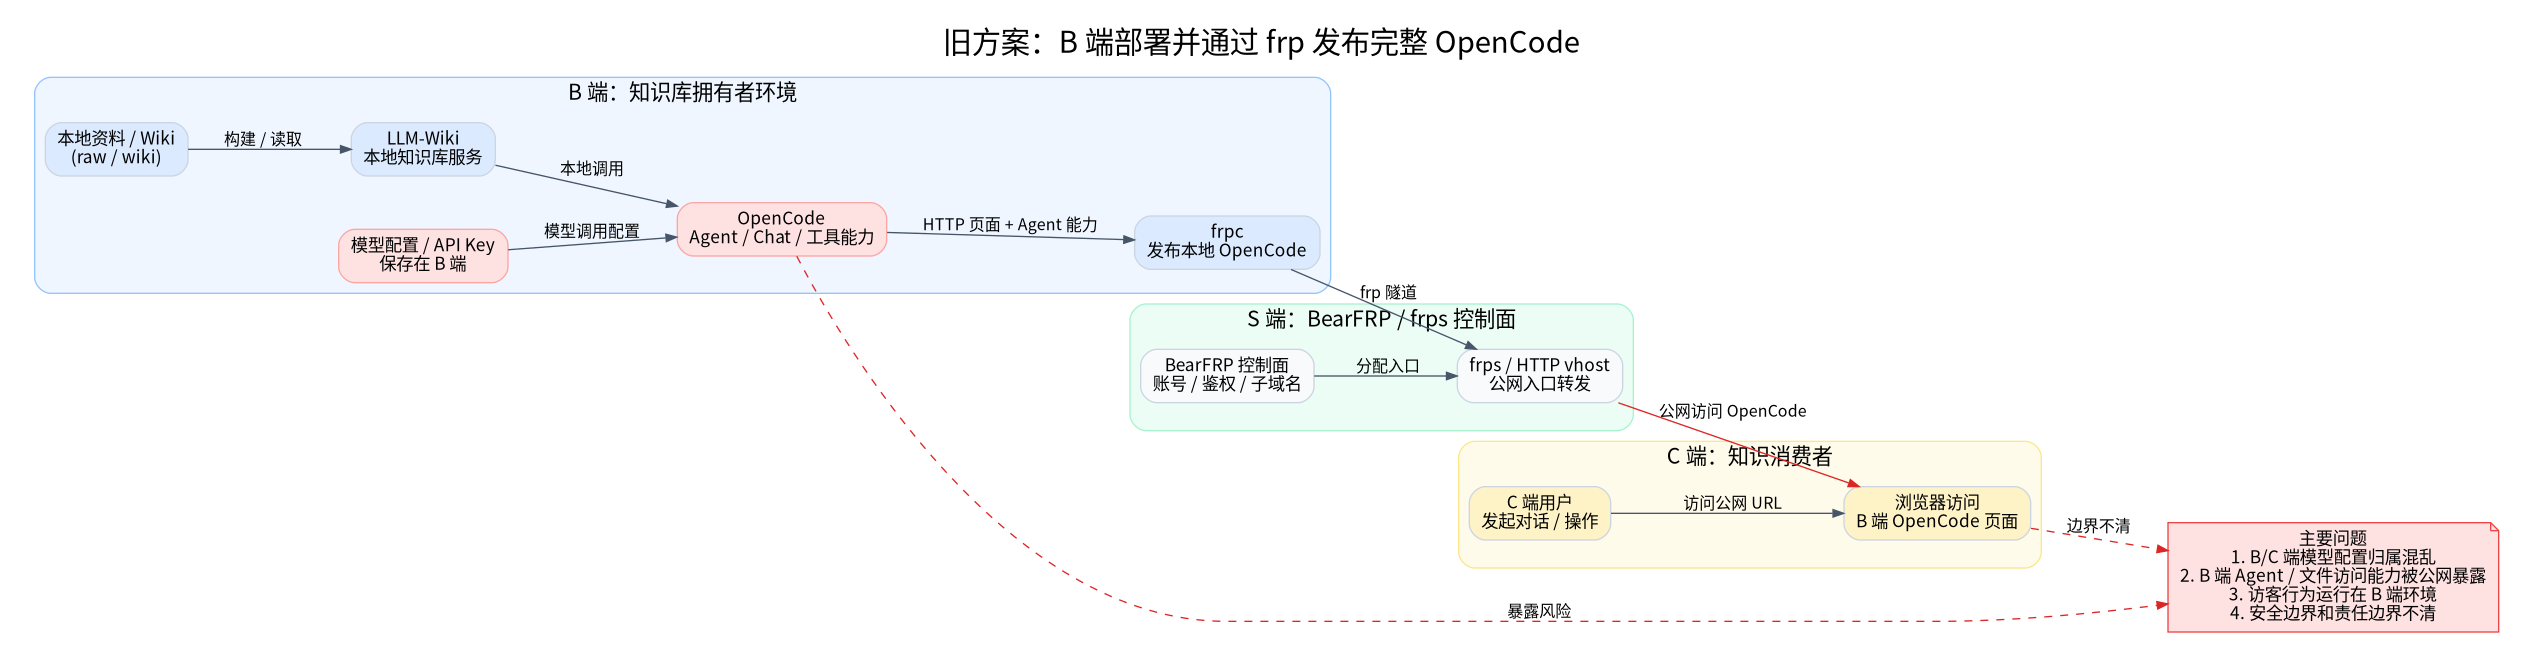
\includegraphics[width=\textwidth]{old_b_side_opencode.png}
  \caption{旧方案架构图：B 端发布完整 OpenCode}
  \label{fig:old-architecture}
\end{figure}

\begin{figure}[H]
  \centering
  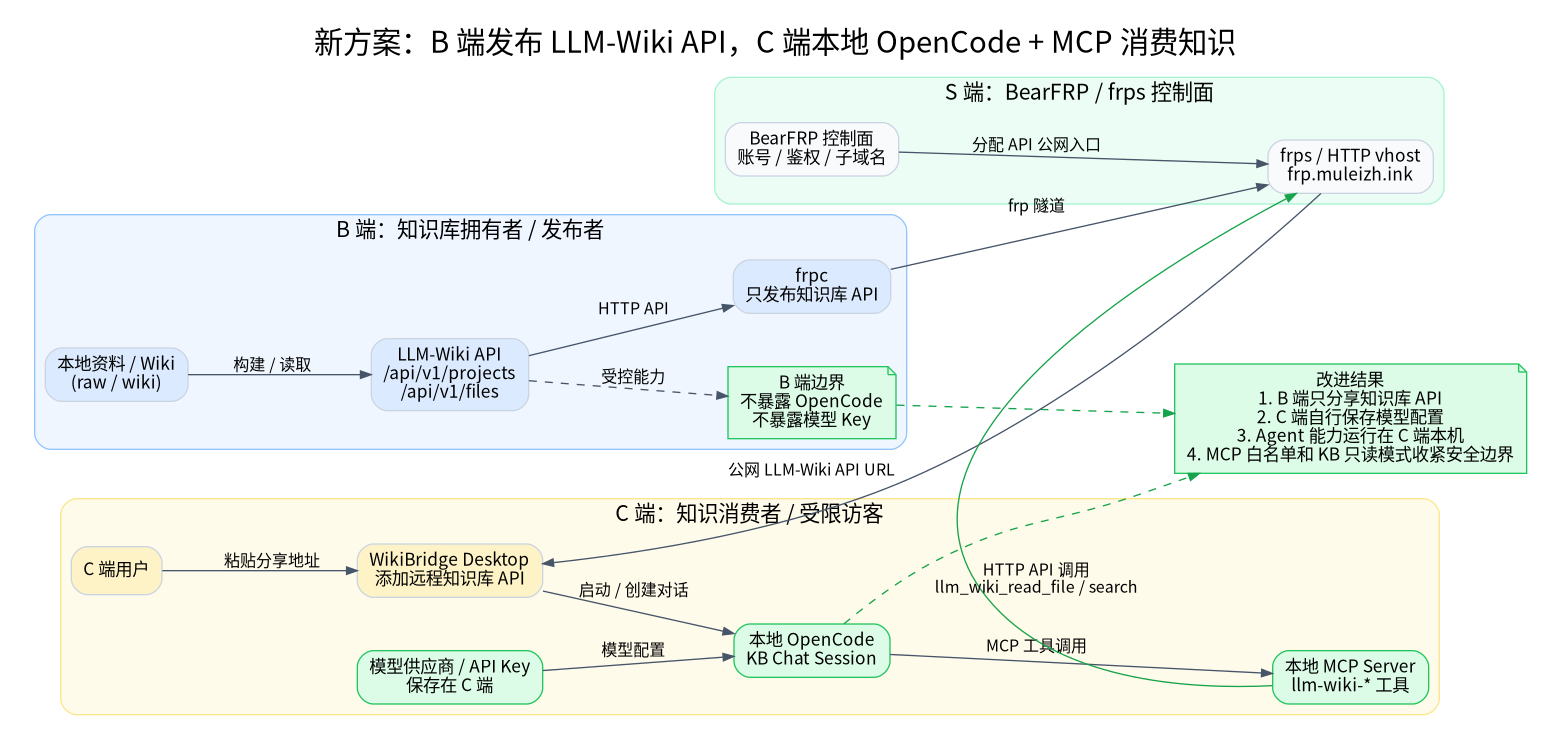
\includegraphics[width=0.96\textwidth]{new_c_side_mcp.png}
  \caption{新方案架构图：C 端本地 OpenCode + MCP}
  \label{fig:new-architecture}
\end{figure}

\subsection{当前总体技术路线}
计划阶段只记录高层技术路线，详细数据流、实体关系、时序图、活动图和部署拓扑迁入后续《软件设计规格说明书》。当前主链路如下：
\begin{enumerate}
  \item B 端本地资料经 LLM-Wiki 构建为 Wiki 项目。
  \item B 端通过 BearFRP/frpc 发布 LLM-Wiki API。
  \item S 端 BearFRP/frps 提供公网入口，例如 \code{*.frp.muleizh.ink}。
  \item C 端在 WikiBridge Desktop 中添加远程知识库 API URL。
  \item C 端本地启动 OpenCode。
  \item C 端注册 \code{llm-wiki-*} MCP。
  \item OpenCode 对话调用 \code{llm_wiki_read_file}、\code{llm_wiki_search} 等工具访问远程知识库。
\end{enumerate}

\subsection{关键设计决策}
\begin{longtable}{>{\bfseries}p{3.2cm}p{4.2cm}p{6.8cm}}
\toprule
决策点 & 选型 & 主要理由 \\
\midrule
知识内容存放 & B 端本地 & 保持本地优先，S 端不托管知识正文。 \\
公网访问 & BearFRP/frp & 适合将本地 API 临时映射到公网。 \\
C 端知识消费 & 本地 OpenCode + MCP & 保持模型配置和 Agent 环境在 C 端。 \\
OpenCode 安全 & KB 只读 + MCP 白名单 & 避免不受控工具能力暴露。 \\
部署方式 & Docker Compose + Desktop sidecar & 课程项目周期内可控，方便演示和联调。 \\
HTTP 发布模式 & 优先真实通配域名；无域名时 TCP 模式 & 避免生成不可解析的子域名 URL。 \\
\bottomrule
\end{longtable}

\subsection{安全边界设计}
OpenCode + MCP 接入的关键安全措施包括：
\begin{itemize}
  \item B 端不发布完整 OpenCode，只发布 LLM-Wiki API。
  \item C 端保存自己的模型 API Key，不依赖 B 端模型配置。
  \item KB 模式下 OpenCode 只允许知识库范围内的受控访问。
  \item \code{OPENCODE_KB_READONLY} 下拒绝写入、修改和删除。
  \item \code{llm-wiki-*} MCP 白名单限制 MCP 名称、命令、入口文件和环境变量。
\end{itemize}

相关实现证据包括 OpenCode KB guard、OpenCode MCP 注册模块、桌面端 sidecar 模块和桌面端联调说明。

\subsection{部署计划}
项目支持两类运行方式：
\begin{enumerate}
  \item Docker Compose 集成演示栈：用于本地和课程验收演示。
  \item B/S/C 分布式联调：B 端运行 LLM-Wiki API，S 端运行 BearFRP/frps，C 端运行 WikiBridge Desktop 和 OpenCode。
\end{enumerate}

关键端口和服务如下：
\begin{longtable}{>{\bfseries}p{4.0cm}>{\centering\arraybackslash}p{2.4cm}p{7.6cm}}
\toprule
服务 & 默认端口 & 说明 \\
\midrule
LLM-Wiki API & 19828 & B 端知识库 API。 \\
OpenCode & 4096 & C 端本地 OpenCode。 \\
BearFRP backend & 8000 & S 端控制面。 \\
frps bind & 7000 & frpc 连接入口。 \\
HTTP vhost & 8080 & HTTP 子域名发布入口。 \\
Desktop dev server & 1420 & Tauri 前端开发入口。 \\
\bottomrule
\end{longtable}

\section{可行性分析}

\subsection{技术可行性}
\begin{longtable}{>{\bfseries}p{3.0cm}p{3.0cm}p{8.2cm}}
\toprule
技术点 & 成熟度评估 & 团队储备/风险 \\
\midrule
LLM-Wiki & 中高 & 已具备本地服务和 API，需继续完善构建流程和测试。 \\
OpenCode & 高 & 上游成熟，但本项目需要 KB 模式和 MCP 接入改造。 \\
MCP & 中高 & 协议适合工具接入，但需要处理注册、白名单和错误提示。 \\
BearFRP/frp & 高 & frp 成熟，BearFRP 控制面需要联调和边界测试。 \\
Tauri/React Desktop & 中高 & 能完成桌面端整合，但跨平台 CI 仍需修复。 \\
Docker Compose & 高 & 适合课程演示和多服务编排。 \\
GitHub Actions CI & 高 & 已有桌面端系统测试，但当前远程知识库 flow 仍有失败项。 \\
\bottomrule
\end{longtable}

关键技术风险与缓解：
\begin{itemize}
  \item HTTP 子域名发布依赖真实通配域名：通过 \code{frp.muleizh.ink} 配置或 TCP 模式规避。
  \item OpenCode 暴露风险：通过架构调整避免 B 端发布 OpenCode。
  \item MCP 工具能力过宽：通过 \code{llm-wiki-*} 白名单和 KB 只读模式限制。
  \item 跨平台桌面测试不稳定：后续修复 CI 和 system mocks。
\end{itemize}

\subsection{经济可行性}
作为课程项目，现金投入较低，主要成本是开发人力和少量服务器/域名资源。

\begin{longtable}{>{\bfseries}p{3.6cm}p{3.0cm}p{7.6cm}}
\toprule
项目 & 估算 & 说明 \\
\midrule
云服务器/VPS & 0--300 元 & 可使用学生额度或组内已有服务器。 \\
域名 & 0--100 元/年 & HTTP 子域名模式建议配置真实域名。 \\
模型 API & 0--少量 & 开发期可使用测试额度。 \\
CI/GitHub & 0 & 使用免费额度。 \\
人力成本 & 不计现金 & 课程项目投入。 \\
\bottomrule
\end{longtable}

若产品化，收益不宜按广告或订阅直接估算。更合理的价值在于降低本地知识库分享门槛，保护未公开资料和科研/课程资料的本地持有权，并支持小组协作、导师临时查看、课程项目交付等有限共享场景。

\subsection{法律与合规可行性}
项目应遵守最小化数据收集和本地优先原则：
\begin{itemize}
  \item S 端只保存账号、鉴权、发布记录、隧道状态等控制面数据。
  \item 不在 S 端存储用户原始资料、Wiki 正文或问答上下文。
  \item C 端模型 API Key 不上传到 S 端。
  \item 对外发布入口应支持关闭、回收和 token 保护。
  \item 公开部署前必须修改默认密码、frps token 和管理员凭据。
\end{itemize}

\subsection{社会与运行可行性}
项目适合以下场景：
\begin{itemize}
  \item 课程小组临时共享项目资料和知识库。
  \item 科研小组分享未公开资料的结构化浏览入口。
  \item 个人将本地笔记整理成 Wiki 后分享给同学或导师查看。
  \item 答辩和演示场景中展示本地知识库的公网访问能力。
\end{itemize}

项目不适合面向全网的公开内容传播、高并发长期内容托管，以及要求搜索引擎收录、评论互动、CDN 分发的博客平台。

\subsection{操作可行性}
B 端用户需要理解的操作应控制在添加资料、构建 Wiki、创建/查看发布入口、分享 API URL。C 端用户需要理解的操作应控制在输入模型 API Key、粘贴远程知识库 API URL、点击连接并在 OpenCode 中提问。因此，系统必须避免让普通用户直接理解 frpc/frps、HTTP vhost、MCP 配置文件等内部细节。

\section{备选方案比较}

\subsection{备选方案 1：B 端发布完整 OpenCode}
该方案最初被考虑：B 端运行完整 OpenCode，通过 frp 将 OpenCode 页面发布给 C 端访问。

优势：
\begin{itemize}
  \item 实现路径直观。
  \item C 端无需安装或启动 OpenCode。
  \item 页面访问链路较短。
\end{itemize}

劣势：
\begin{itemize}
  \item B/C 端模型配置归属混乱。
  \item B 端 Agent、文件访问和工具能力被公网暴露。
  \item C 端访客行为运行在 B 端环境。
  \item 安全边界不清。
\end{itemize}

结论：不采用。

\subsection{备选方案 2：B 端只发布静态 Wiki 页面}
该方案只发布渲染后的 Wiki 页面，不提供 C 端 OpenCode/MCP 对话能力。

优势：
\begin{itemize}
  \item 安全风险最低。
  \item 实现简单。
  \item 对 C 端要求低，只需浏览器。
\end{itemize}

劣势：
\begin{itemize}
  \item 缺少对话式知识消费能力。
  \item 项目亮点不足。
  \item 不能体现 OpenCode/MCP 集成价值。
\end{itemize}

结论：可作为降级方案，但不是主方案。

\subsection{备选方案 3：B 端发布 LLM-Wiki API，C 端本地 OpenCode + MCP}
该方案为当前主方案。

优势：
\begin{itemize}
  \item B 端不暴露完整 OpenCode。
  \item C 端保存自己的模型配置。
  \item Agent 能力运行在 C 端本地。
  \item B/S/C 三端职责清晰。
  \item 可通过 MCP 白名单和 KB 只读模式收紧安全边界。
\end{itemize}

劣势：
\begin{itemize}
  \item C 端需要启动本地 OpenCode。
  \item MCP 注册、桌面端状态管理和错误提示更复杂。
  \item 自动化测试和 CI 覆盖成本更高。
\end{itemize}

结论：采用。

\subsection{方案对比总结}
\begin{longtable}{>{\bfseries}p{3.0cm}p{3.5cm}p{3.2cm}p{4.0cm}}
\toprule
维度 & B 端发布 OpenCode & 只发布静态 Wiki & C 端 OpenCode + MCP \\
\midrule
安全边界 & 差 & 优 & 良好 \\
C 端体验 & 中 & 中 & 优 \\
Agent 能力 & 有但风险高 & 无 & 有且边界清晰 \\
实现复杂度 & 中 & 低 & 高 \\
课程技术深度 & 中 & 低 & 高 \\
最终选择 & 不采用 & 降级方案 & 主方案 \\
\bottomrule
\end{longtable}

\section{投入与效益分析}

\subsection{项目投入}
\begin{longtable}{>{\bfseries}p{3.2cm}p{3.0cm}p{8.0cm}}
\toprule
投入项 & 估算 & 说明 \\
\midrule
服务器 & 0--300 元 & BearFRP/frps 需要公网服务器。 \\
域名 & 0--100 元 & HTTP 子域名模式推荐配置通配域名。 \\
模型 API & 少量 & 开发和演示阶段可控。 \\
开发人力 & 6 人课程小组 & 按 LLM-Wiki、BearFRP/frp、OpenCode/Chatbox、Desktop、MCP、CI 与测试等方向投入。 \\
测试与文档 & 课程实验周期内完成 & 覆盖实验 5、实验 6、终版分组报告和个人总结材料。 \\
\bottomrule
\end{longtable}

\subsection{项目收益}
\begin{itemize}
  \item 完成本地知识库生成、发布和 C 端对话式消费闭环。
  \item 验证 BearFRP + LLM-Wiki + OpenCode + MCP 的集成可行性。
  \item 形成可展示的课程项目原型。
  \item 沉淀 B/S/C 三端架构、MCP 接入和 KB 安全边界设计经验。
  \item 为个人和小团队的有限知识共享提供原型参考。
\end{itemize}

\subsection{风险与敏感性}
\begin{longtable}{>{\bfseries}p{3.8cm}p{2.2cm}p{4.0cm}p{4.0cm}}
\toprule
风险 & 影响 & 缓解措施 & 说明 \\
\midrule
通配域名未配置 & HTTP 子域名 URL 不可解析 & 配置真实域名，或使用 TCP 发布模式。 & 影响演示入口可用性。 \\
OpenCode 直接暴露 & B 端安全风险扩大 & 采用 C 端本地 OpenCode + MCP。 & 已通过架构调整规避。 \\
模型 API 配置缺失 & C 端无法对话 & 桌面端提供模型配置入口和明确提示。 & 需在验收前验证。 \\
MCP 注册失败 & OpenCode 无法访问远程知识库 & 检查 MCP 状态、提供重试和错误提示。 & 属于核心链路风险。 \\
CI 跨平台失败 & 质量保障不完整 & 修复 desktop system mocks，补回归测试。 & 需保留手工验证路径。 \\
frpc/frps 连接不稳定 & 公网入口不可用 & 健康检查、日志、重连和手工验证。 & 与网络环境相关。 \\
默认凭据未修改 & 公开部署安全风险 & 公开部署前强制修改密码和 token。 & 发布前必须处理。 \\
\bottomrule
\end{longtable}

\section{项目开发计划}

\subsection{工作内容综述}
项目开发工作按六个阶段组织：
\begin{enumerate}
  \item 需求与架构确认。
  \item 原型与核心模块开发。
  \item BearFRP 发布链路开发。
  \item LLM-Wiki / OpenCode / MCP 集成。
  \item 端到端联调与测试。
  \item 文档、演示和验收交付。
\end{enumerate}

\subsection{工作分解结构}
\begin{longtable}{>{\bfseries}p{3.0cm}p{5.8cm}p{5.4cm}}
\toprule
阶段 & 工作内容 & 关键产物 \\
\midrule
需求与架构 & 用户角色、B/S/C 架构、边界和风险确认。 & SRS、架构图、计划书。 \\
知识库模块 & LLM-Wiki 构建、API、项目/文件/搜索能力。 & LLM-Wiki API。 \\
发布控制面 & BearFRP 用户、代理、余额、脚本、frps/frpc。 & BearFRP 控制面。 \\
桌面端集成 & WikiBridge Desktop、远程知识库、OpenCode 启停。 & Desktop。 \\
OpenCode + MCP & KB 模式、MCP 注册、只读和白名单。 & OpenCode/MCP 集成。 \\
部署与 CI & Docker Compose、sidecar、系统测试、CI。 & 部署说明、测试脚本。 \\
测试与文档 & 黑盒/白盒、联调缺陷、验收材料。 & 测试文档、PPT、总结。 \\
\bottomrule
\end{longtable}

\begin{figure}[H]
\centering
\resizebox{\textwidth}{!}{%
\begin{tikzpicture}[
  font=\tiny,
  root/.style={draw=whu, thick, rounded corners=4pt, fill=softblue, align=center, minimum width=3.2cm, minimum height=0.75cm},
  phase/.style={draw=whu, thick, rounded corners=3pt, fill=white, align=center, minimum width=2.2cm, minimum height=0.72cm},
  work/.style={draw=linegray, rounded corners=2pt, fill=softgray, align=center, minimum width=2.0cm, minimum height=0.56cm},
  flow/.style={draw=whu, thick}
]
\node[root] (root) at (0,0) {WikiBridge 项目开发};
\foreach \x/\name/\id in {-7.2/需求与架构/a,-4.8/知识库模块/b,-2.4/发布控制面/c,0/桌面端集成/d,2.4/OpenCode + MCP/e,4.8/部署与 CI/f,7.2/测试与文档/g} {
  \node[phase] (p\id) at (\x,-1.25) {\name};
  \draw[flow] (root.south) |- (p\id.north);
}
\node[work] at (-7.2,-2.35) {用户角色\\场景};
\node[work] at (-7.2,-3.05) {B/S/C\\边界};
\node[work] at (-4.8,-2.35) {Wiki\\构建};
\node[work] at (-4.8,-3.05) {项目/文件\\搜索 API};
\node[work] at (-2.4,-2.35) {用户/余额\\代理};
\node[work] at (-2.4,-3.05) {HTTP/TCP\\发布入口};
\node[work] at (0,-2.35) {远程知识库\\添加};
\node[work] at (0,-3.05) {OpenCode\\启停};
\node[work] at (2.4,-2.35) {KB Session};
\node[work] at (2.4,-3.05) {MCP 注册\\白名单};
\node[work] at (4.8,-2.35) {Compose\\部署};
\node[work] at (4.8,-3.05) {CI\\回归};
\node[work] at (7.2,-2.35) {联调缺陷};
\node[work] at (7.2,-3.05) {验收文档};
\foreach \x in {-7.2,-4.8,-2.4,0,2.4,4.8,7.2} {
  \draw[flow] (\x,-1.62) -- (\x,-2.05);
}
\end{tikzpicture}}
\caption{WikiBridge 工作分解结构图}
\label{fig:wbs}
\end{figure}

\subsection{人员组织与分工}
以下分工按终版联调和提交材料归纳，只记录主要方向，实际开发中存在跨模块讨论、联调和共同修正。

\begin{longtable}{>{\bfseries}p{2.6cm}p{5.2cm}p{6.4cm}}
\toprule
成员 & 主要方向 & 说明 \\
\midrule
陈明德 & OpenCode + MCP 接入、跨端联调、BearFRP 相关开发 & 已完成 C 端本地 OpenCode + MCP 访问远程 LLM-Wiki API 的联调。 \\
郭一言 & Wiki 方向、frp 模块及联调相关工作 & 负责 Wiki 相关集成，并参与 frp 发布链路联调。 \\
张沐雷 & 持续集成 CI、桌面端测试/自动化相关 & 负责 GitHub Actions 持续集成、桌面端测试和自动化测试支撑。 \\
骆贝尔 & LLM-Wiki 方向 & 负责 LLM-Wiki 相关功能和知识库生成能力。 \\
曾浩正 & OpenCode / Chatbox 方向 & 负责 OpenCode / Chatbox 相关知识消费能力。 \\
童济舟 & OpenCode / Chatbox 方向 & 参与 OpenCode / Chatbox 方向开发与联调。 \\
\bottomrule
\end{longtable}

\subsection{协作机制}
\begin{itemize}
  \item 代码仓库：Git/GitHub。
  \item 沟通方式：线下讨论、IM 群组和 Git 提交记录。
  \item 分支策略：当前仍需规范化，建议后续采用 feature branch + 小粒度提交。
  \item Code Review：目前没有正式 PR Review，后续建议至少对大功能合并做轻量评审。
  \item 测试策略：联调测试 + 系统测试 + CI 回归 + 实验 5 黑盒/白盒测试。
\end{itemize}

\subsection{进度安排}
以下按课程项目实际推进节奏整理。

\begin{longtable}{>{\bfseries}p{3.2cm}p{2.5cm}p{8.3cm}}
\toprule
阶段 & 周期 & 里程碑 \\
\midrule
M1 需求与计划 & W1 & 完成计划书、SRS 初稿、分工确认。 \\
M2 架构设计 & W2 & 完成 SDS、B/S/C 架构图、关键接口设计。 \\
M3 核心开发 & W3--W5 & 完成 LLM-Wiki、BearFRP、Desktop、OpenCode/MCP 核心开发。 \\
M4 联调演示 & W5--W6 & 跑通 B 端 API 发布、C 端 OpenCode + MCP 访问链路。 \\
M5 测试完成 & W6 & 完成实验 5 黑盒/白盒测试和 CI 修复。 \\
M6 验收交付 & W7 & 完成测试文档、部署说明、答辩 PPT、个人总结。 \\
\bottomrule
\end{longtable}

\begin{figure}[H]
\centering
\resizebox{\textwidth}{!}{%
\begin{tikzpicture}[
  font=\scriptsize,
  grid/.style={draw=linegray, line width=0.3pt},
  task/.style={draw=whu, fill=softblue, rounded corners=2pt, minimum height=0.42cm},
  taskb/.style={draw=whu, fill=softgreen, rounded corners=2pt, minimum height=0.42cm},
  taskc/.style={draw=whu, fill=softorange, rounded corners=2pt, minimum height=0.42cm},
  axis/.style={draw=whu, thick}
]
\def\x0{4.35}
\def\w{1.55}
\foreach \i/\week in {0/W1,1/W2,2/W3,3/W4,4/W5,5/W6,6/W7} {
  \node[font=\bfseries\color{whu}] at (\x0+\i*\w+0.75,0) {\week};
  \draw[grid] (\x0+\i*\w,-0.35) -- (\x0+\i*\w,-6.65);
}
\draw[grid] (\x0+7*\w,-0.35) -- (\x0+7*\w,-6.65);
\draw[axis] (\x0,-0.35) -- (\x0+7*\w,-0.35);
\foreach \y/\name in {
  -0.95/{项目定位与角色确认},
  -1.65/{计划书与 SRS 初稿},
  -2.35/{B/S/C 架构图与方案对比},
  -3.05/{SDS 与接口边界},
  -3.75/{LLM-Wiki、BearFRP、Desktop、MCP 核心开发},
  -4.45/{B/S/C 端到端联调},
  -5.15/{实验 5 黑盒/白盒测试与 CI 修复},
  -5.85/{部署说明、PPT 与个人总结}
} {
  \node[anchor=east, align=right, text width=4.4cm] at (4.1,\y) {\name};
}
\node[task, minimum width=1.05cm] at (\x0+0.38,-0.95) {};
\node[task, minimum width=1.35cm] at (\x0+1.05,-1.65) {};
\node[taskb, minimum width=1.35cm] at (\x0+1.65,-2.35) {};
\node[taskb, minimum width=1.65cm] at (\x0+2.35,-3.05) {};
\node[taskc, minimum width=4.85cm] at (\x0+3.55,-3.75) {};
\node[taskb, minimum width=2.2cm] at (\x0+5.15,-4.45) {};
\node[taskc, minimum width=1.95cm] at (\x0+5.65,-5.15) {};
\node[task, minimum width=1.95cm] at (\x0+6.35,-5.85) {};
\end{tikzpicture}}
\caption{WikiBridge 项目周级甘特图}
\label{fig:gantt}
\end{figure}

\subsection{验收标准}
\subsubsection{功能完整度}
\begin{itemize}
  \item B 端能生成本地 Wiki。
  \item B 端能通过 BearFRP 发布 LLM-Wiki API。
  \item C 端能添加远程知识库 API。
  \item C 端能启动本地 OpenCode 并注册 \code{llm-wiki-*} MCP。
  \item C 端能在 OpenCode 对话中读取或搜索远程知识库。
\end{itemize}

\subsubsection{安全边界}
\begin{itemize}
  \item B 端不暴露完整 OpenCode。
  \item C 端模型 API Key 不上传到 S 端。
  \item OpenCode KB 模式和 MCP 白名单生效。
  \item 公开部署前默认密码和 token 已替换。
\end{itemize}

\subsubsection{测试要求}
\begin{itemize}
  \item BearFRP 用户与代理测试覆盖注册、登录、充值、代理创建、删除和脚本生成。
  \item 桌面端系统测试覆盖远程知识库 flow。
  \item 实验 5 补充黑盒测试和白盒控制流图。
  \item CI 中关键测试通过或对失败项有明确修复计划。
\end{itemize}

\subsubsection{文档要求}
\begin{itemize}
  \item 计划书、需求规格说明书、软件设计规格说明书、测试文档、部署说明和交接说明齐备。
  \item 架构图体现旧方案与新方案对比。
  \item 个人总结能引用截图、提交号、测试编号和文件路径。
\end{itemize}

\subsection{风险与应对}
\begin{longtable}{p{3.6cm}>{\centering\arraybackslash}p{1.3cm}>{\centering\arraybackslash}p{1.3cm}p{4.7cm}p{3.1cm}}
\toprule
风险描述 & 可能性 & 影响 & 应对措施 & 责任人 \\
\midrule
HTTP 子域名缺少通配域名 & 中 & 高 & 配置真实域名 \code{frp.muleizh.ink} 或切换 TCP 发布。 & 发布链路负责人 \\
B 端 OpenCode 暴露风险 & 中 & 高 & 改为 C 端本地 OpenCode + MCP。 & OpenCode 与 MCP 负责人 \\
MCP 注册失败 & 中 & 中 & 增加状态展示、错误提示和重试。 & Desktop 与 OpenCode 负责人 \\
CI 跨平台失败 & 中 & 中 & 修复 mocks，拆分测试，保留手工验证路径。 & CI 负责人 \\
提交粒度过粗 & 中 & 中 & 后续按功能拆分提交，轻量 Review。 & 全体 \\
文档滞后 & 高 & 中 & 计划书、SRS、SDS 与测试文档并行补齐。 & 文档负责人 \\
模型 API 不可用 & 中 & 中 & 提供配置入口和错误提示，保留无模型降级说明。 & LLM-Wiki 与 OpenCode 负责人 \\
\bottomrule
\end{longtable}

\section{支持条件}

\subsection{开发环境}
\begin{itemize}
  \item 操作系统：Linux / macOS / Windows。
  \item IDE：VS Code 或 JetBrains 系列。
  \item Node.js：项目当前桌面端开发使用 Node 22 相关环境。
  \item Rust/Tauri：用于桌面端。
  \item Python/FastAPI：用于 BearFRP 控制面。
  \item Docker Compose：用于集成部署。
  \item Git/GitHub：用于版本管理和 CI。
\end{itemize}

\subsection{测试环境}
\begin{itemize}
  \item 本地 Docker Compose 环境。
  \item GitHub Actions 桌面端 CI。
  \item BearFRP 公网服务器和真实域名。
  \item 本地 C 端 OpenCode 环境。
\end{itemize}

\subsection{运行环境}
\begin{itemize}
  \item B 端：运行 LLM-Wiki API、frpc、知识库数据目录。
  \item S 端：运行 BearFRP backend、frps、控制面数据。
  \item C 端：运行 WikiBridge Desktop、OpenCode、MCP server。
\end{itemize}

\subsection{组内支持条件}
\begin{itemize}
  \item 需要组内统一最终分工表。
  \item 需要补齐 SRS 和 SDS。
  \item 需要为实验 5 预留黑盒/白盒测试时间。
  \item 需要在验收前确认所有截图、Git 记录、CI 状态和部署说明。
\end{itemize}

\section{结论与建议}
综合分析，WikiBridge 在课程项目周期内具备可行性。项目所依赖的 LLM-Wiki、OpenCode、MCP、frp、Docker Compose 等技术均有可用基础，核心难点不在单点技术是否存在，而在跨模块集成、三端职责边界和安全控制。

项目已经明确从旧方案“B 端发布完整 OpenCode”调整为新方案“B 端发布 LLM-Wiki API，C 端本地 OpenCode + MCP”。该调整降低了 B 端安全风险，明确了模型配置归属，也更符合有限共享的产品定位。

建议后续重点推进：
\begin{enumerate}
  \item 补齐需求规格说明书和软件设计规格说明书，将 B/S/C 三端最终架构写入正式文档。
  \item 完成实验 5 黑盒/白盒测试，特别是远程知识库、OpenCode 启动、MCP 注册和 BearFRP 发布链路。
  \item 修复桌面端远程知识库 flow 的 CI 失败项。
  \item 规范提交粒度和轻量 Code Review，避免大功能一次性提交影响追溯。
  \item 在课程项目中期或类似项目后续迭代中增加最小端到端链路演示，允许展示半成品但要求说明已闭环、mock 和待完善内容。
\end{enumerate}

\appendix
\section{终版材料索引}
\begin{itemize}
  \item WikiBridge 软件需求规格说明书。
  \item WikiBridge 软件设计说明书。
  \item WikiBridge 测试分析报告。
  \item WikiBridge 终版分组实习报告。
\end{itemize}

\section{可引用证据}
\begin{longtable}{>{\bfseries}p{3.2cm}p{11.0cm}}
\toprule
证据 & 说明 \\
\midrule
WikiBridge Desktop 交接说明 & 当前架构说明。 \\
WikiBridge 部署说明 & 部署和 BearFRP 发布说明。 \\
端到端联调截图 & C 端本地 OpenCode 调用 \code{llm_wiki_read_file} 读取远程知识库。 \\
远程知识库流程 CI 截图 & 远程 Wiki flow 系统测试 CI 失败截图。 \\
\code{bab897616} & \code{fix: enable OpenCode KB chat sessions}。 \\
\code{62e049539} & \code{fix: share llm wiki api for desktop remotes}。 \\
\code{816554778} & \code{docs: add desktop handoff startup guide}。 \\
\code{cee791768} & \code{test: update desktop system mocks for remote wiki flow}。 \\
\bottomrule
\end{longtable}

\end{document}
